\section{Introduction}\label{sec:intro}
\IEEEPARstart{R}{obots} that work with people ask them questions. A service robot asks which object is meant before it grasps; a collaborative robot asks whether the person is ready before it hands over a tool; a robot that learns from feedback asks which of two trajectories is better~\cite{Christiano2017}. Help-seeking planners make asking an explicit decision: the robot acts when its plan is unambiguous and asks when it is not~\cite{Ren2023,Yuan2026}, and interactive imitation learning decides when to hand control to a person under a budget~\cite{Hoque2021}. In all of these systems the answer is treated as a reading of a fixed belief that the person already holds.

Human judgement does not behave that way. Answers depend on the order in which questions are asked: in a Gallup poll of September 1997, 50\% of respondents called Bill Clinton honest when asked about him first, but 57\% did so after a question about Al Gore, while Gore's rating fell from 68\% to 60\% in the reverse order~\cite{Moore2002}. Asking a question can also change what a person thinks next. In a motion-detection task, an intermediate judgement changed later judgements in a way that Markov models of belief change could not reproduce~\cite{Kvam2015,Busemeyer2019}. Quantum-like (quantum-probability) models represent these effects by treating a belief as a vector and a question as a projection; they predict order effects, a parameter-free regularity called the QQ equality~\cite{Wang2013b,Wang2014}, and interference between judgements~\cite{Busemeyer2012,Pothos2013a,Pothos2022}. They have been proposed for trust in automation and in human--AI teams~\cite{Roeder2023,Humr2023,Lawless2020}, but a companion systematic review found almost no tests of such models in robots or agents~\cite{Guru2026b}.

This paper asks three questions. Can a quantum-like model of a person's answers be told apart from classical alternatives with the amount of data a robot study can collect? What does a robot gain by using it, and what does it lose if the model is wrong? Does asking about trust change trust, and can the robot tell whether it does? The contributions are:
\begin{itemize}
\item an order-aware human model for robot questioning, built from a three-dimensional quantum-like question model with projector ranks, three classical baselines and two trust-dynamics models (Markov and open-system), implemented and tested in open code;
\item simulation studies in three robot domains (object clarification, trust and hand-over, preference elicitation) of model recovery, cross-order prediction and questioning design, with homogeneous and heterogeneous populations;
\item a trust study showing how a question about trust can change later trust, how many people are needed to detect it, and what error a robot makes if it ignores it;
\item a test against two published data sets (the Clinton--Gore poll and the Prisoner's Dilemma disjunction effect~\cite{Shafir1992});
\item quantum-circuit versions of both models, verified on simulators and under the noise models of current IBM quantum processors, with scripts for IBM Quantum and Amazon Braket.
\end{itemize}
Fig. \ref{fig:framework} summarizes the approach. The model also supplies a confidence signal for the learned orchestrator reviewed in a companion survey~\cite{Guru2026s3}: the predictive uncertainty about a person's answer or trust (Section \ref{sec:robot}).

\begin{figure*}[!t]
\centering
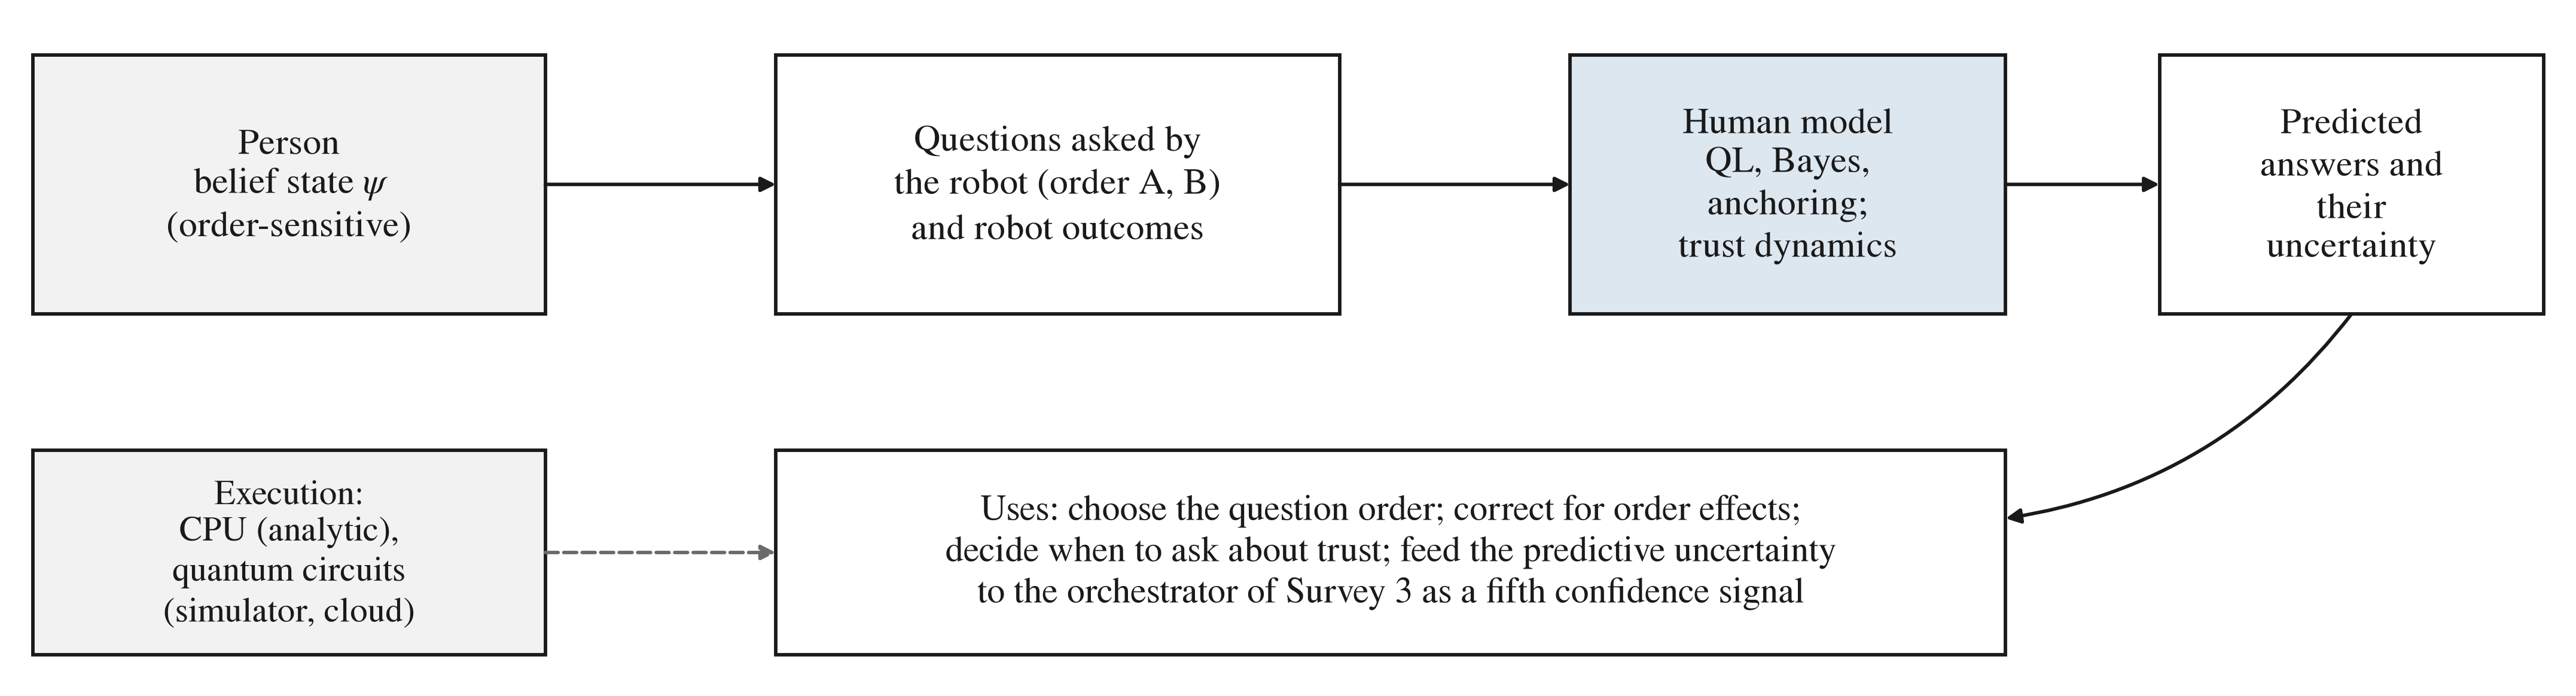
\includegraphics[width=\textwidth]{figures/Fig1_framework.png}
\caption{Approach. The robot's questions and its hand-over outcomes act on the person's belief state; competing human models (quantum-like, Bayesian, anchoring; open-system and Markov trust) predict the answers and their uncertainty, which the robot uses to choose and order its questions and passes to its orchestrator as a confidence signal. The models run analytically on a CPU or as quantum circuits.}\label{fig:framework}
\end{figure*}


\section{Background}\label{sec:background}
\subsection{Order Effects and the QQ Equality}
Let two yes/no questions $A$ and $B$ be asked in either order, and let $p_{AB}(y,n)$ be the probability of answering yes to $A$ and then no to $B$. A classical model in which answers read out a fixed joint distribution gives the same marginal probability to each question whatever its position, so it has no order effect. Order effects can be added classically, for example by letting the first answer anchor the second~\cite{Trueblood2011}. Quantum-like models predict order effects from the geometry of the questions and satisfy, for any parameters, the QQ equality
\begin{equation}
p_{AB}(y,n)+p_{AB}(n,y)=p_{BA}(y,n)+p_{BA}(n,y),\label{eq:qq}
\end{equation}
which was supported across 70 national field experiments on question order~\cite{Wang2014}. Classical models do not satisfy (\ref{eq:qq}) in general, although some do: an anchoring model with one shared weight does, and so do order-free Bayesian models trivially. Models of probability judgement with noise also produce related regularities~\cite{Costello2014,Costello2018}, and the QQ equality alone is not proof of quantum-like processing~\cite{BoyerKassem2016,Khrennikov2014,Ozawa2021}.

\subsection{Trust Dynamics}
Trust in automation grows with reliable performance and falls after failures~\cite{Lee2004}. Markov models describe trust as a probability over hidden states that is updated by outcomes; a question about trust reads the state and, averaged over the answer, leaves it unchanged. Quantum-like models of trust calibration~\cite{Roeder2023,Humr2023} and of belief change~\cite{Busemeyer2019} allow superposed states whose coherence is lost by measurement, so that asking can change what follows.


\section{Models}\label{sec:models}
\subsection{Quantum-Like Question Model}\label{sec:ql}
The person's belief is a unit vector $\psi\in\mathbb{R}^3$, and a yes answer to question $q$ is a projector $P_q$ onto either the ray of a unit vector $u_q$ (rank 1) or the plane orthogonal to it (rank 2). Answering applies the L\"uders rule~\cite{Busemeyer2012}: $p(\text{yes})=\|P_q\psi\|^2$, after which $\psi\leftarrow P_q\psi/\|P_q\psi\|$ (and the complement for no). Up to a rotation, the model has three angles,
\begin{equation}
\begin{aligned}
\psi&=e_1,\quad u_A=(\cos a,\sin a,0),\\
u_B&=(\cos b,\sin b\cos g,\sin b\sin g),
\end{aligned}
\end{equation}
plus the discrete ranks of the two yes subspaces. A two-dimensional model has only two effective parameters and cannot fit the Clinton--Gore pattern: when half the respondents answer the first question with yes, it forces the second-position rate to 0.5. The three-dimensional model with ranks (1, 2) fits it (Section \ref{sec:lit}).

\subsection{Classical Baselines}\label{sec:classical}
\textit{Bayes} is an order-free joint distribution with marginals $p_A$, $p_B$ and a correlation parameter (three parameters); response noise added to it remains in this family. \textit{Anchoring} gives the first answer at its first-position rate and pulls the second answer toward the first: $P(y_2\mid y_1)=p_2+w_q(1-p_2)$ and $P(y_2\mid n_1)=p_2(1-w_q)$ for $w_q\ge 0$ (contrast for $w_q<0$), where $q$ is the second question. With one weight (Anchoring1, three parameters) it satisfies (\ref{eq:qq}); with a weight per question (Anchoring2, four parameters) it does not. A \textit{saturated} model with a free distribution for each order (six parameters) is a reference.

\subsection{Trust Models}\label{sec:trustmodels}
A person observes a sequence of robot hand-overs with outcomes $o_t\in\{1,0\}$ (success, failure). The \textit{Markov} model has $P(\text{trust})$ initially $p_0$; after a success, distrust becomes trust with probability $s$; after a failure, trust becomes distrust with probability $f$. The \textit{open-system} model is a qubit density matrix $\rho$ with $|0\rangle$ for trust, initialized by a rotation $R_y(\phi_0)$. After a success it applies $R_y(-\alpha_s)$, after a failure $R_y(\alpha_f)$, and then dephasing of strength $\gamma$, which multiplies the off-diagonal entries by $1-\gamma$ (a Lindblad dephasing channel over one step). A trust question is a projective measurement in the trust basis. With $\gamma=1$ the model loses all coherence and behaves like a Markov chain; with $\gamma<1$ an intermediate question removes coherence that would otherwise have interfered with later rotations, so asking changes later trust.

\subsection{Robot Domains and Simulated People}\label{sec:domains}
Three domains fix a pair of questions and the size of the order effect (Fig. \ref{fig:orders}): \textit{object clarification} (``Is it the red cup?'', ``Is it the cup on the left?''), with an assimilation effect as large as in the Clinton--Gore poll; \textit{trust and hand-over} (``Do you trust the robot to hand you the tool?'', ``Was the last hand-over safe?''), with a smaller assimilation effect; and \textit{preference elicitation} (``Is trajectory 1 acceptable?'', ``Is trajectory 2 acceptable?''), with a contrast effect. For each domain, four synthetic populations generate answers: \textit{QL} (the quantum-like model fitted to the target rates); \textit{Anchoring} (the two-weight model with the same first- and second-position rates where it can reach them, so the two generators differ only in their joint structure); \textit{Bayes} (an order-free model with the QL model's A-first joint distribution); and \textit{Mixture} (half QL, half anchoring). Populations are either homogeneous or heterogeneous: in the latter, each of 2,000 simulated people draws its own parameters around the population values with a spread of 0.1 (radians for angles; logit or weight units otherwise). The target rates are illustrative choices, not estimates from people. Each simulated person answers both questions once, in one order.

\begin{figure*}[!t]
\centering
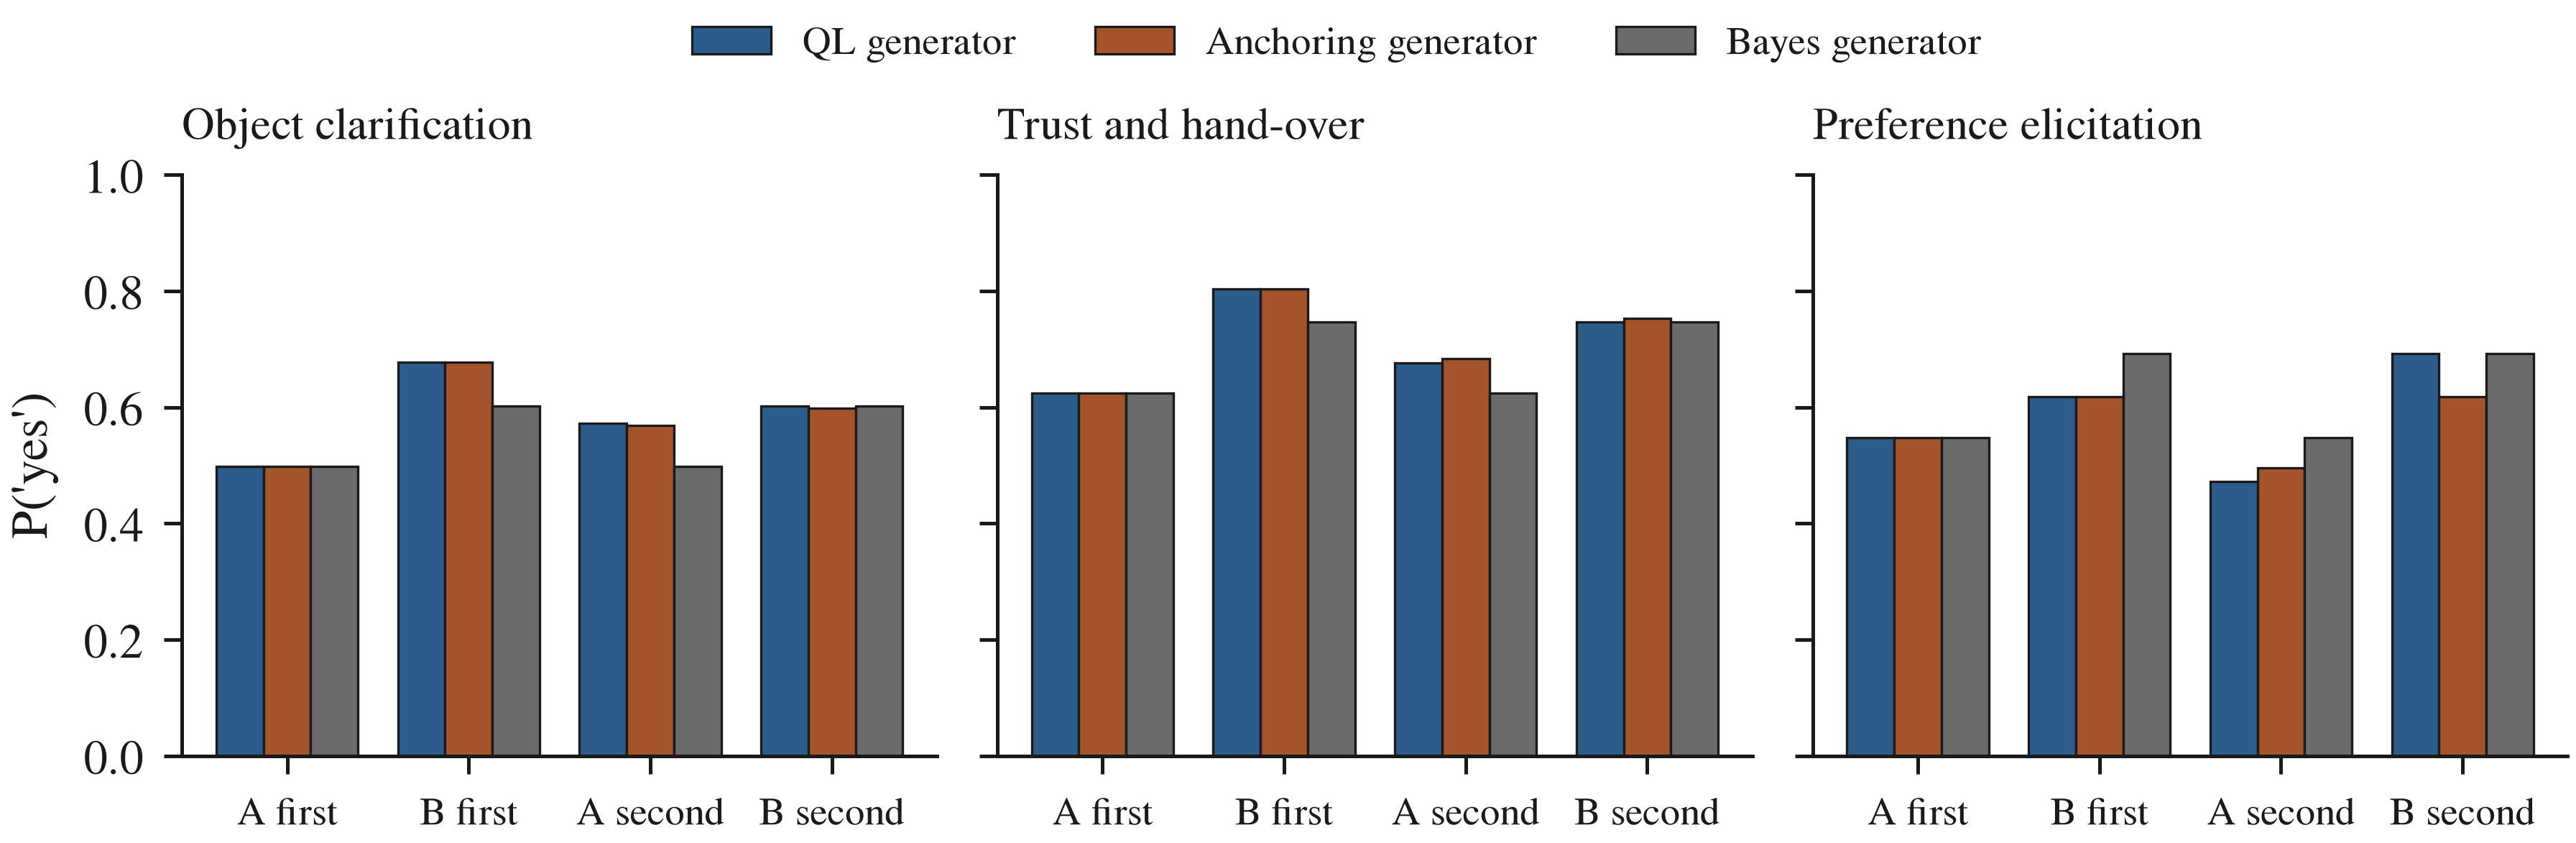
\includegraphics[width=\textwidth]{figures/Fig2_order_effects.png}
\caption{Answer rates of the synthetic populations in the three domains: probability of a yes answer to each question when it is asked first or second. QL and anchoring share these rates (except the second-position rate of B in preference elicitation, which anchoring cannot reach); Bayes has no order effect.}\label{fig:orders}
\end{figure*}


\section{Experimental Method}\label{sec:method}
\textit{Fitting and selection.} Models are fitted by maximum likelihood to answer counts (Nelder--Mead with eight random restarts; for the QL model, every rank combination). Models are compared by the Bayesian information criterion (BIC), and the QQ equality is tested with a two-sided $z$ test at $\alpha=0.05$.

\textit{Experiment 1 (model recovery).} For each domain, generator, population type and sample size (100, 400 or 1,600 people per order), answers in both orders are simulated, the QL, Bayes and Anchoring2 models are fitted, and the model with the lowest BIC is recorded; 30 repetitions per condition.

\textit{Experiment 2 (cross-order prediction).} Training data are $N$ people answering A then B ($N$ = 400 or 4,000) plus a probe of $N/10$ answering B then A. Each model predicts the B-first answer distribution; the score is the Kullback--Leibler divergence from the generator's true B-first distribution (median over 30 repetitions).

\textit{Experiment 3 (questioning design).} The robot must learn the first-position (``unprimed'') yes rates $\pi_A$ and $\pi_B$ from 400 people who each answer both questions. Designs: a fixed order AB with $\pi_B$ read from the second answers, as a robot that ignores order effects would do; a probe of 10\% or 30\% of people answering B first, with a model fitted to all answers; and a split design (half each order) using only first answers, which needs no model. With the order fixed, $\pi_B$ is not identifiable under the QL model: two parameter sets reproduce the AB answers exactly but imply different $\pi_B$ (for object clarification, 0.525 and 0.678); the probe resolves this. Score: root-mean-square error (RMSE) of $\pi_B$ over 30 repetitions.

\textit{Experiment 4 (trust).} Six hand-overs with outcomes (1, 1, 0, 1, 0, 1). In condition C0 the robot asks about trust only after the sixth hand-over; in C1 also after the third. The generators are the open-system model ($\phi_0=1.6$, $\alpha_s=0.8$, $\alpha_f=1.2$, $\gamma=0.3$; illustrative values) and the Markov model that best matches it. Both models are fitted to C0 and C1 answers with 100, 400 or 1,600 people per condition and compared by BIC. A robot that has only C1 data (it always asks midway) predicts the trust it would have found without the midway question; the RMSE of that prediction measures the cost of assuming that asking has no effect. 30 repetitions.

\textit{Experiment 5 (published data).} The models are fitted by least squares to the four Clinton--Gore rates~\cite{Moore2002,Wang2013b}; only aggregate proportions are available, so likelihoods are not computed. For the Prisoner's Dilemma~\cite{Shafir1992}, the classical law of total probability and the quantum-like law with an interference term are compared~\cite{Pothos2009}.

\textit{Experiment 6 (circuits).} The question circuits for each domain and order and the trust circuits for both conditions are run with 20,000 shots on the Qiskit Aer simulator~\cite{JavadiAbhari2024} (ideal, and with the noise models of the IBM FakeTorino and FakeBrisbane backends) and on the Amazon Braket local simulators (ideal, and with depolarizing noise of 0.5\% and 2\% after every gate). The scores are the total variation distance (TVD) between the circuit's and the analytic answer distributions and the QQ value of the circuit output.

\textit{Circuit design.} The belief space is embedded in two qubits ($e_1=|00\rangle$, $e_2=|01\rangle$, $e_3=|10\rangle$). To ask question $q$, a Householder reflection $V_q$ maps $u_q$ to $|00\rangle$; an ancilla is flipped if and only if the system is in $|00\rangle$ (a Toffoli gate between $X$ gates); only the ancilla is measured, which implements the binary L\"uders measurement without collapsing the no subspace; $V_q$ is then applied again. The trust circuit uses one qubit with $R_y$ rotations, and dephasing is applied by an ancilla that triggers a $Z$ gate with probability $\gamma/2$ and is then reset. Each circuit has a dynamic form (mid-circuit measurement and reset) and a deferred form in which every measurement is copied to a fresh ancilla and read at the end~\cite{Nielsen2010}; the latter runs on hardware without mid-circuit measurement.
